
\documentclass{article}

% Packages for formatting
\usepackage[margin=1in]{geometry}
\usepackage{fancyhdr}
\usepackage{enumitem}
\usepackage{graphicx}
\usepackage{kotex}
\usepackage{amsmath}
\usepackage{amsthm}
\usepackage{algorithm2e,setspace}
\usepackage{algpseudocode}
\usepackage{xcolor}
\usepackage{amssymb}

% Fonts
\usepackage[T1]{fontenc}
\usepackage[utf8]{inputenc}
\usepackage{newpxtext,newpxmath}
\usepackage{sectsty}

% Define colors
\definecolor{blue1}{HTML}{0077c2}
\definecolor{blue2}{HTML}{00a5e6}
\definecolor{blue3}{HTML}{b3e0ff}
\definecolor{blue4}{HTML}{00293c}
\definecolor{blue5}{HTML}{e6f7ff}
\definecolor{titleblue}{RGB}{0,53,128}
\definecolor{chaptergray}{RGB}{140,140,140}
\definecolor{sectiongray}{RGB}{180,180,180}


\definecolor{thmcolor}{RGB}{231, 76, 60}
\definecolor{defcolor}{RGB}{52, 152, 219}
\definecolor{lemcolor}{RGB}{155, 89, 182}
\definecolor{corcolor}{RGB}{46, 204, 113}
\definecolor{procolor}{RGB}{241, 196, 15}

\usepackage{color,soul}
\usepackage{soul}
\newcommand{\mathcolorbox}[2]{\colorbox{#1}{$\displaystyle #2$}}
\usepackage{cancel}
\newcommand\crossout[3][black]{\renewcommand\CancelColor{\color{#1}}\cancelto{#2}{#3}}
\newcommand\ncrossout[2][black]{\renewcommand\CancelColor{\color{#1}}\cancel{#2}}

\usepackage{hyperref}

% Chapter formatting
\definecolor{titleblue}{RGB}{0,53,128}
\usepackage{titlesec}
\titleformat{\section}
{\normalfont\sffamily\Large\bfseries\color{titleblue!100!gray}}{\thesection}{1em}{}
\titleformat{\subsection}
{\normalfont\sffamily\large\bfseries\color{titleblue!50!gray}}{\thesubsection}{1em}{}

%Tcolorbox
\usepackage[most]{tcolorbox}

%Tikzpicture
\usepackage{tikz-cd}
\usetikzlibrary{positioning}

\usepackage{pgfplots}
\pgfplotsset{compat=1.17}

\newcommand{\ie}{\textnormal{i.e.}}
\newcommand{\rsa}{\mathsf{RSA}}
\newcommand{\rsacrt}{\mathsf{RSA}\textendash\mathsf{CRT}}
\newcommand{\inv}[1]{#1^{-1}}

% Header and footer formatting
\pagestyle{fancy}
\fancyhead{}
\fancyhf{}
\rhead{Student ID: 20192250\quad Name: 지용현}%\rule{3cm}{0.4pt}}
\lhead{\textcolor{blue2}{\textbf{2023-1st-semester Seminar \#1}}}
% Define footer
\newcommand{\footer}[1]{
\begin{flushright}
	\vspace{2em}
	\includegraphics[width=2cm]{school_logo.jpg} \\
	\vspace{1em}
	\textcolor{blue2}{\small\textbf{#1}}
\end{flushright}
}
%\rfoot{\large Department of Information Security, Cryptogrphy and Mathematics, Kookmin Uni.\includegraphics[height=1.5cm]{school_logo.jpg}}
\fancyfoot{}
\fancyfoot[C]{-\thepage-}

\usepackage{amsthm}
\newtheorem{axiom}{Axiom}[section]
\newtheorem{theorem}{Theorem}
\newtheorem*{theorem*}{Theorem}
\newtheorem{proposition}[theorem]{Proposition}
\newtheorem{corollary}{Corollary}[theorem]
\newtheorem*{corollary*}{Corollary}
\newtheorem{lemma}[theorem]{Lemma}
\newtheorem*{lemma*}{Lemma}

\theoremstyle{definition}
\newtheorem{definition}{Definition}
\newtheorem*{definition*}{Definition}
\newtheorem{remark}{Remark}
\newtheorem{exercise}{Exercise}[section]

%New Command
\newcommand{\set}[1]{\left\{#1\right\}}
\newcommand{\N}{\mathbb{N}}
\newcommand{\Z}{\mathbb{Z}}
\newcommand{\Q}{\mathbb{Q}}
\newcommand{\R}{\mathbb{R}}
\newcommand{\C}{\mathbb{C}}
\newcommand{\F}{\mathbb{F}}
\newcommand{\nbhd}{\mathcal{N}}

\newcommand{\of}[1]{\left( #1 \right)}

\begin{document}
\pagenumbering{arabic}
\begin{center}
	\huge\textbf{How to Find Root Values:}\\
	\Large\textit{Newton-Raphson and Binary Methods}\\
	\vspace{0.5em}
\end{center}

\section{Introduction}

We will discuss two methods for finding the square root of a number, specifically the square root of 2. These methods are the Newton-Raphson method and the Binary method. We will provide a mathematical explanation for each method and include graphs to illustrate the process, using the function $f(x) = x^2 - 2$ as an example.

\section{Newton-Raphson Method}

The Newton-Raphson method is an iterative numerical method used to find the roots of a real-valued function. Given a function $f(x)$ and its derivative $f'(x)$, the method starts with an initial guess $x_0$ and iteratively refines the guess using the following formula:

\[
x_{n+1} = x_n - \frac{f(x_n)}{f'(x_n)}
\]

In our case, $f(x) = x^2 - 2$, and its derivative is $f'(x) = 2x$. Thus, the iterative formula for finding the square root of 2 becomes:

\[
x_{n+1} = x_n - \frac{x_n^2 - 2}{2x_n} = \frac{x_n + \frac{2}{x_n}}{2}
\]

\begin{figure}[ht]
	\centering
	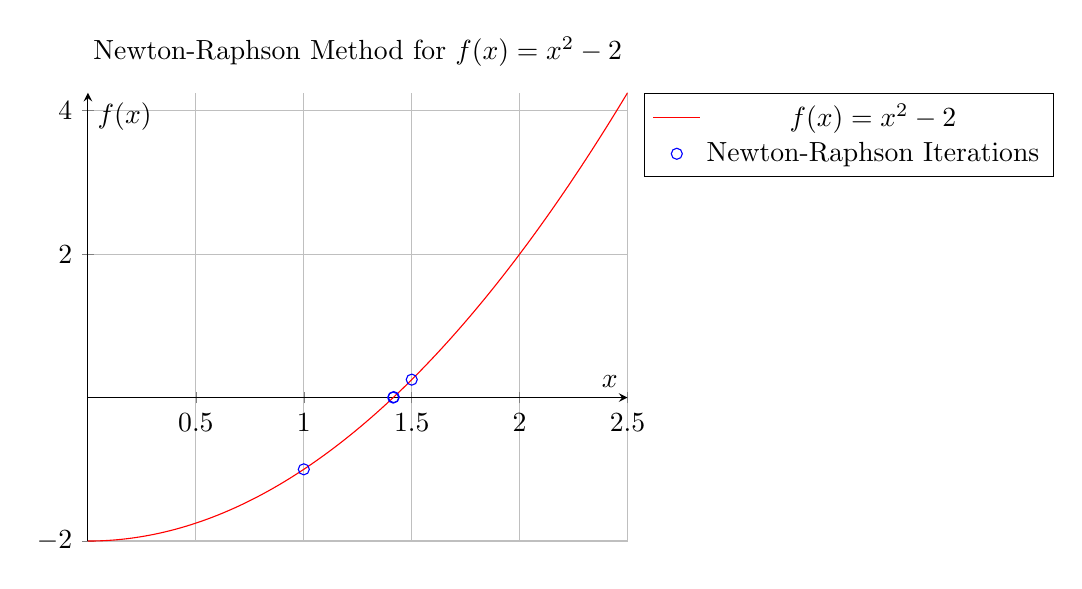
\begin{tikzpicture}
		\begin{axis}[
			title={Newton-Raphson Method for $f(x) = x^2 - 2$},
			xlabel={$x$},
			ylabel={$f(x)$},
			grid=major,
			axis lines=center,
			legend pos=outer north east,
			]
			\addplot[red, domain=0:2.5, samples=100] {x^2 - 2};
			\addlegendentry{$f(x) = x^2 - 2$}
			\addplot[blue, only marks, mark=o] coordinates {(1, -1) (1.5, 0.25) (1.4167, 0.0069) (1.4142, 0.00002)};
			\addlegendentry{Newton-Raphson Iterations}
		\end{axis}
	\end{tikzpicture}
	\caption{Newton-Raphson method applied to $f(x) = x^2 - 2$.}
\end{figure}

\section{Binary Method}

The Binary method, also known as the Bisection method, is another iterative numerical method to find the roots of a real-valued function. This method relies on the Intermediate Value Theorem, which states that if a continuous function takes on two values $f(a)$ and $f(b)$ with different signs, then it must take on the value 0 in the interval $(a, b)$.

The Binary method works by narrowing down the interval containing the root. It starts with an interval $[a, b]$ such that $f(a) < 0$ and $f(b) > 0$. The midpoint of the interval is calculated as $c = \frac{a+b}{2}$. If $f(c) = 0$, then $c$ is the root of the function. If $f(c) < 0$, then the new interval is $[c, b]$. If $f(c) > 0$, then the new interval is $[a, c]$. The process is repeated until the desired level of accuracy is achieved or the maximum number of iterations is reached.

For the function $f(x) = x^2 - 2$, we start with an interval $[1, 2]$ since $f(1) = -1$ and $f(2) = 2$. The Binary method will iteratively narrow down the interval containing the square root of 2.

\begin{figure}[ht]
	\centering
	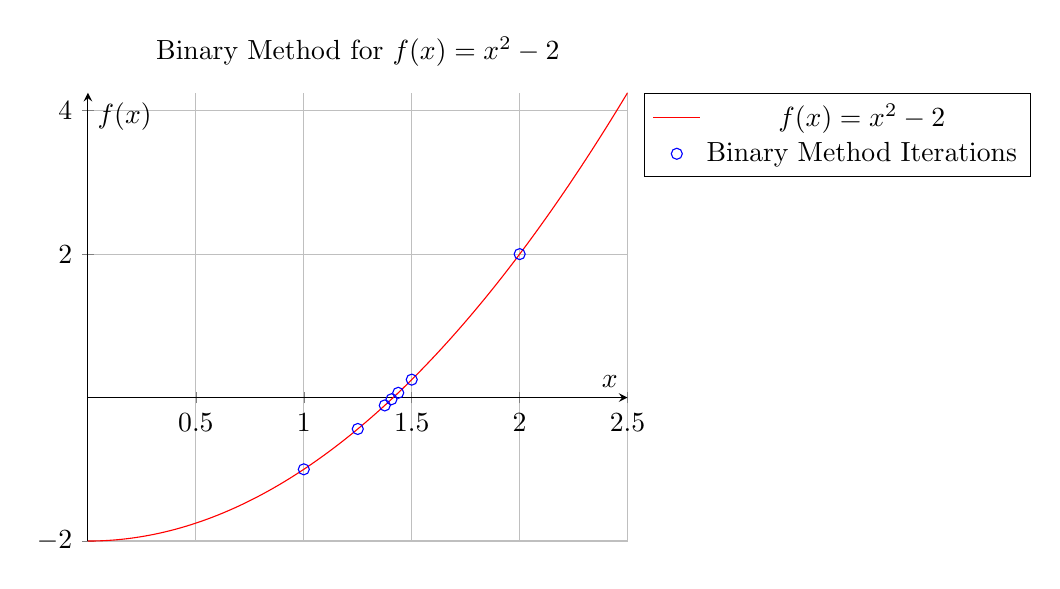
\begin{tikzpicture}
		\begin{axis}[
			title={Binary Method for $f(x) = x^2 - 2$},
			xlabel={$x$},
			ylabel={$f(x)$},
			grid=major,
			axis lines=center,
			legend pos=outer north east,
			]
			\addplot[red, domain=0:2.5, samples=100] {x^2 - 2};
			\addlegendentry{$f(x) = x^2 - 2$}
			\addplot[blue, only marks, mark=o] coordinates {(1, -1) (2, 2) (1.5, 0.25) (1.25, -0.4375) (1.375, -0.1094) (1.4375, 0.0664) (1.4063, -0.0232)};
			\addlegendentry{Binary Method Iterations}
		\end{axis}
	\end{tikzpicture}
	\caption{Binary method applied to $f(x) = x^2 - 2$.}
\end{figure}

\section{Conclusion}

We have discussed two methods for finding the square root of a number, specifically the square root of 2: the Newton-Raphson method and the Binary method. We provided a mathematical explanation for each method and illustrated the process using graphs for the function $f(x) = x^2 - 2$. Both methods can be used to approximate the square root of a number, with the choice of method depending on the specific problem and desired level of accuracy.



\footer{Department of Information Security, Cryptography and Mathematics\\ Kookmin University}
\end{document}
